\usetikzlibrary{patterns}


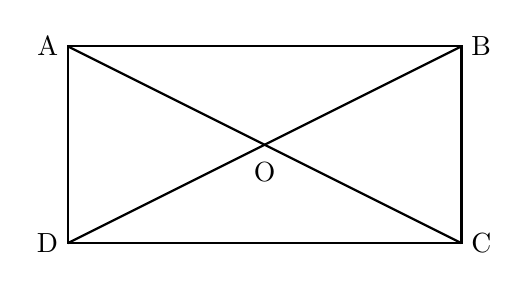
\begin{tikzpicture}[scale=1]

    % Define the coordinates for the vertices of the rectangle
    \coordinate (D) at (0,0);
    \coordinate (C) at (5,0);
    \coordinate (B) at (5,2.5);
    \coordinate (A) at (0,2.5);

    % Define the coordinate for the intersection of the diagonals
    \coordinate (O) at (2.5,1.25);

    % Draw the main rectangle (ABCD)
    \draw[thick] (A) -- (B) -- (C) -- (D) -- cycle;

    % Draw the diagonals (AC and BD)
    \draw[thick] (A) -- (C);
    \draw[thick] (D) -- (B);

    % Label the vertices exactly as shown in the image
    \node[left] at (A) {A};
    \node[right] at (B) {B};
    \node[right] at (C) {C};
    \node[left] at (D) {D};

    % Label the center point O
    \node[below, yshift=-0.1cm] at (O) {O};

\end{tikzpicture}